
\chapter{Product description: AsthmaBuddy}
\label{chp:our-solution}

\section{Background}
In 2012, we did a similar project using Karotz \fnurl{Karotz}{www.karotz.com} as our platform \cite{CustomerDriven}. The thought behind Karotz is great. It is an open source robot which allows people to build applications and launch it to the Karotz store. However, in our subjective opinion, it is not ideal to work with. The Karotz starters kit costs ~\$200, not including customs, thus it is a pretty large investment for a family wanting to buy the product to use with our application. The API is only documented in French, which makes it a hassle, in addition to the fact that it is pretty cumbersome to configure for a ``non-technological'' family. 


We have looked around for other options to create our tangible user interface, i.e. Arduino and Raspberry Pi. Arduino is an open source electronics prototyping platform \cite{arduino}, which allows for many different combinations of configurations, while \rpi{} is a cheap computer on the size of a credit card. Arduino shields comes in many shapes and sizes and is built for modularity and extendability. A wide-range of components are available if you want to add technical functionality to an Arduino system, such as Bluetooth, WiFi or small motors. 
While Arduino allows complex hardware configurations, Raspberry Pi makes larger abstractions, which seemed like the better choice for us as developers. Arduino programs are normally written in C \cite{strahl2000language}, and while there exists many tutorials and manuals for how to write Arduino code, we found the thought of writing in a programming language we hade little prior knowledge of too challenging. Arduinos generally have low-powered CPUs, in order to keep them cheap. These low-powered CPUs tend to have problems with decoding MP3-files, which would lay constraints on our system. Due to these facts, we choose to develop the system on a Raspberry Pi.


\subsection{Raspberry Pi}
The \rpi{} was initially intended to teach british school children about computer programming \cite{rasperrypi-about}. Since its release, it took an unexpected turn when lots of computer enthusiasts bought the product to do their own mini projects for a cheap price. 

The specification of a \rpi{} (Model B) is included in Table \ref{tab:pi-specs}. Figure \ref{fig:pi-arch-overview} shows an overview of the \rpi{}.        

\begin{table}
\begin{tabular}{|p{6.0cm} | p{6.0cm} |}
\hline 
\textbf{Property} & \textbf{Specification} \\
\hline
CPU & 700 MHz ARM1176JZF-S core \\
\hline
Memory & 512 MB \\
\hline
USB 2.0 ports & 2 \\
\hline
Video Output & HDMI \\
\hline
Audio Output & 3.5 mm jack, in addition to ability to play sound through HDMI \\
\hline
Low-level Peripherals & 8 x GPIO (General Purpose Input/Output) \\
\hline
Power Source & 5 volt MicroUSB \\
\hline
Storage & SD card (available with preinstalled OS) \\
\hline
Network & 10/100 Mbps Ethernet.  \\
\hline
\end{tabular}
\caption{Raspberry Pi specifications}
\label{tab:pi-specs}
\end{table}

\begin{figure}[H] 
	\centering
		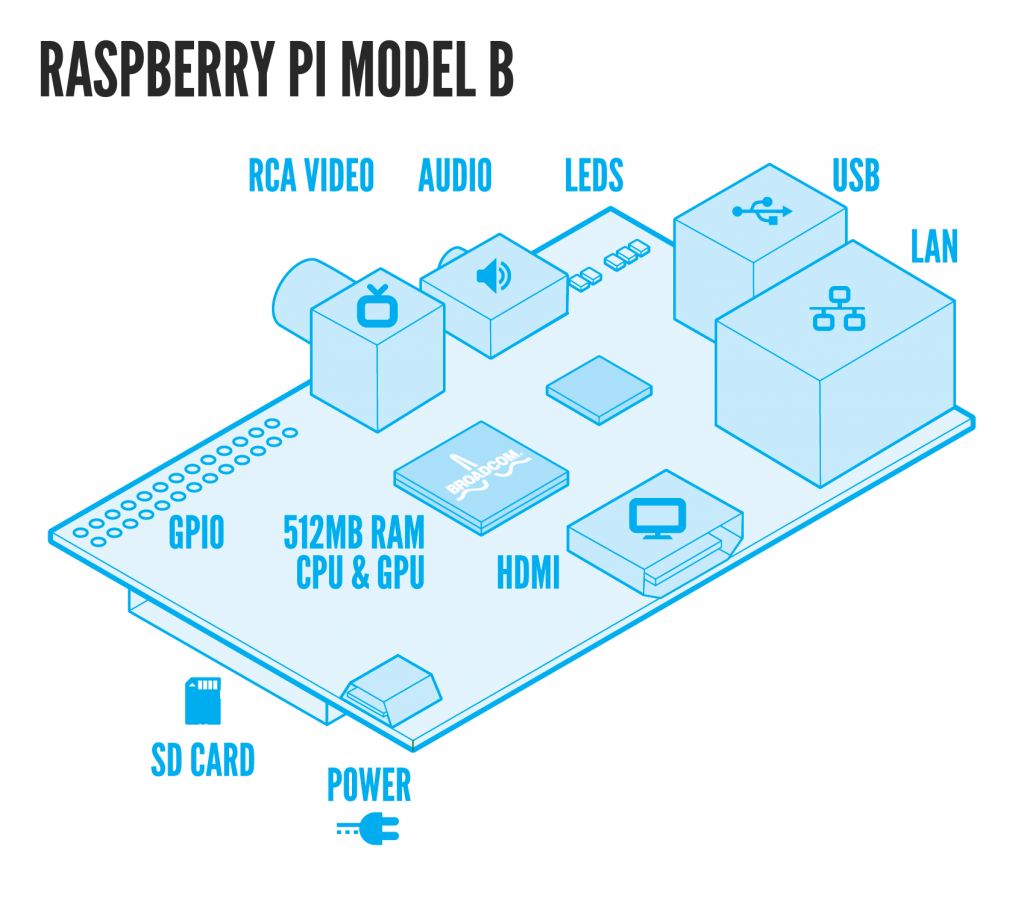
\includegraphics[width=0.6\paperwidth]{Pictures/rpi-arch-overview.png}
	\caption{Raspberry Pi Model B architecture. \emph{Image source: http://raspberrypi.org/faqs} }
	\label{fig:pi-arch-overview}
\end{figure}
 
  
\subsection{Components}
In addition to the \rpi{} we needed some components that children are able to interact through. These components and their functionality are summarized in this section. 


\paragraph{RFID Reader}
A child needs to be able to interact with AsthmaBuddy. We identified two approaches; using a button and/or using RFID technology to do it. We figured that having a big button on the top of a teddy bear would seem somewhat unnatural for a child. Additionally, this could cause problems with the wires inside the teddybear, as a child pushing a button could imply that AsthmaBuddy would be moved around. This could have been avoided by using a battery pack for the \rpi{}, but their capacity does not seem to exceed 24 hours when the \rpi{} is in idle mode. The conclusion was to use RFID technology to proceed in the medication process.


The RFID reader we used was a Sparkfun ID-12LA \fnurl{Sparkfun ID-12LA documentation}{http://dlnmh9ip6v2uc.cloudfront.net/datasheets/Sensors/ID/ID-2LA,\%20ID-12LA,\%20ID-20LA(2013-4-10).pdf}. One of the requirements of the USB reader was that it should be able to connect through an USB-port. 
         
\paragraph{USB speakers}
In order to play sounds to children, we decided to integrate speakers inside AsthmaBuddy. Since we did not want to pull too many wires out of the bear, we decided to use USB-powered speakers.    

\paragraph{LED lights}
We used LED lights connected to a breadboard in order to play around with the first prototype. The LED lights emits light in different colors to correspond to what action(s) is expected from the user during a treatment (see more in INSERT REFERENCE TO PROTOTYPE 1).

\paragraph{Pi4j}
Pi4j\fnurl{Pi4j}{http://pi4j.com} is a Java framework that allows development for \rpi{} in Java, without having to write anything in C. 

\section{Use Cases}
Figure \ref{fig:pi-use-cases} shows a general overview of the use cases we have included in our prototype. A medication process can be started in one out of two ways. 
A parent can register an alarm by using AsthmAPP. This alarm is then triggered by AsthmaBuddy, giving the child a notification that it is time to take their medicine.

The alternative is if children need to take their medicine by need. If they need to take a medicine by need, they simply register their RFID-tag before children are taken through a quicker process (see Manuscript \ref{chp:anuscript}).  

\begin{figure}[H] 
	\centering
		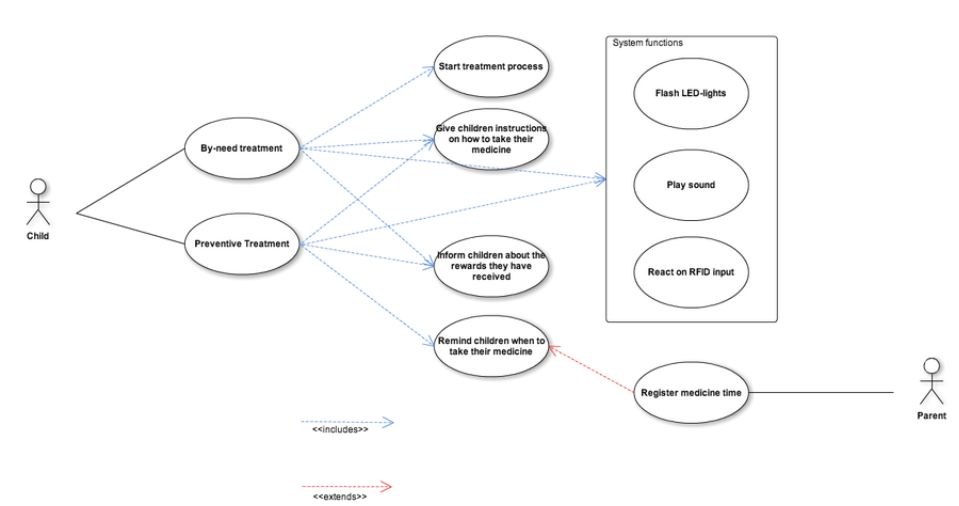
\includegraphics[width=0.8\paperwidth]{Pictures/usecases.png}
	\label{fig:pi-use-cases}
	\caption{AsthmaBuddy Use Cases}
\end{figure}

\subsection{Textual Use Cases}

%--------- TEXTUAL USE CASE ----------
%--------- BY NEED TREATMENT ---------
\begin{table}[H]
\begin{tabular}{|p{4.0cm} | p{9.0cm} |}
\hline
\textbf{Title} & By need treatment \\
\hline
\textbf{Preconditions} & - \\
\hline 
\textbf{Scenario} & 
	\begin{enumerate}
	  \item User triggers treatment by registering RFID-tag
	  \item System plays sound to instruct (Shake the medicine)
	  \item System flashes LED-lights to notify user
	  \item System plays sound to instruct user (Mount medicine in mask, and put mask on)
	  \item User starts a treatment by using RFID-tag
	  \item System plays sound to count during treatment (1-2-3-4-5-6-7-8-9-10), while flashing lights for each count
	  \item System plays sound to tell user he/she has done a good job (Well done)
	  \item System calculates reward based on health state
	  \item System plays sound to award user
	\end{enumerate}
\\
\hline
	\textbf{Extensions} & 
		x.a User aborts treatment by not continuing the sequence
\\
\hline
\end{tabular}
\caption{Textual use case: By need treatment}
\label{tab:textual-use-case}
\end{table}


%--------- PREVENTIVE TREATMENT -------
\begin{table}[H]
\begin{tabular}{|p{4.0cm} | p{9.0cm} |}
\hline
\textbf{Title} & By need treatment \\
\hline
\textbf{Preconditions} & A reminder has been fired \\
\hline 
\textbf{Scenario} & 
	\begin{enumerate}
	  \item Child registers RFID-tag, to notify that he/she is ready
	  \item Start instructions by playing sound (It is time to take medicine. Retrieve the medicine)
	  \item Receive input from RFID-tag
	  \item System plays sound to instruct user (shake the medicine)
	  \item Receive input from RFID-tag
	  \item System plays sound to instruct user
	  \item System starts counting to 10. 
	  \item System plays sound to tell the user he/she has done a good job
	  \item System calculates reward based on health state
	  \item System plays sound to award user
	\end{enumerate}
\\
\hline
	\textbf{Extensions} & 
		x.a Child does not register the RFID-tag when prompted
\\
\hline
\end{tabular}
\caption{Textual use case: By need treatment}
\label{tab:textual-use-case}
\end{table} 


\section{Design Rationale}
When designing \buddy{} we choose to use a teddy bear as an avator for our system. There are several reasons as to why we think this is an appropriate avatar. Teddy bears are well known toys, and has been loved for a long time. They are considered gender-neutral \cite{stagnitti1997determining} \cite{cherney2006gender} and in our subjective opinion it is a toy that could be discretely placed in a children's room. With the look of a teddy bear, \buddy{} can easily be placed among other toys and not be too visible. It was also important for us to choose a teddy bear of some size. A too thin bear could lead to problems with fitting the system inside the bear, and could in order lead to scepticism from the children. 

While designing our system we also wanted to make sure our system did not have robot-like features or robotic similarities. While children tend to find technology very interesting, we want to make \buddy{} seem as natural as possible, making a stuffed animal buddy, rather than a technological toy. We believe that these design choices serves our purpose of making children more aware of their asthma, while not being a constant reminder and a stress element.

Norwegian fire fighters have used a teddy bear in order to calm down children who find themselves in dramatic situations \fnurl{NRK: Firefighters use teddy bears to calm down children}{http://www.nrk.no/trondelag/bamser-i-utrykningsbilene-1.11548966}. The fire fighters state that the children respond positively to the teddy bear. 
While we were not able to find scientific research done on the use of teddy bears in dramatic situations, we found this news article interesting and a relevant mention to our research.

[Pictures of the bear we chose?]


\section{State Diagram}
When the \rpi{} boots, it retrieves the latest version of the source code from Git, compiles it, and starts running it. If a child approaches \buddy{} and registers a RFID-tag, a medication sequence is started.  

\begin{figure}[H] 
	\centering
		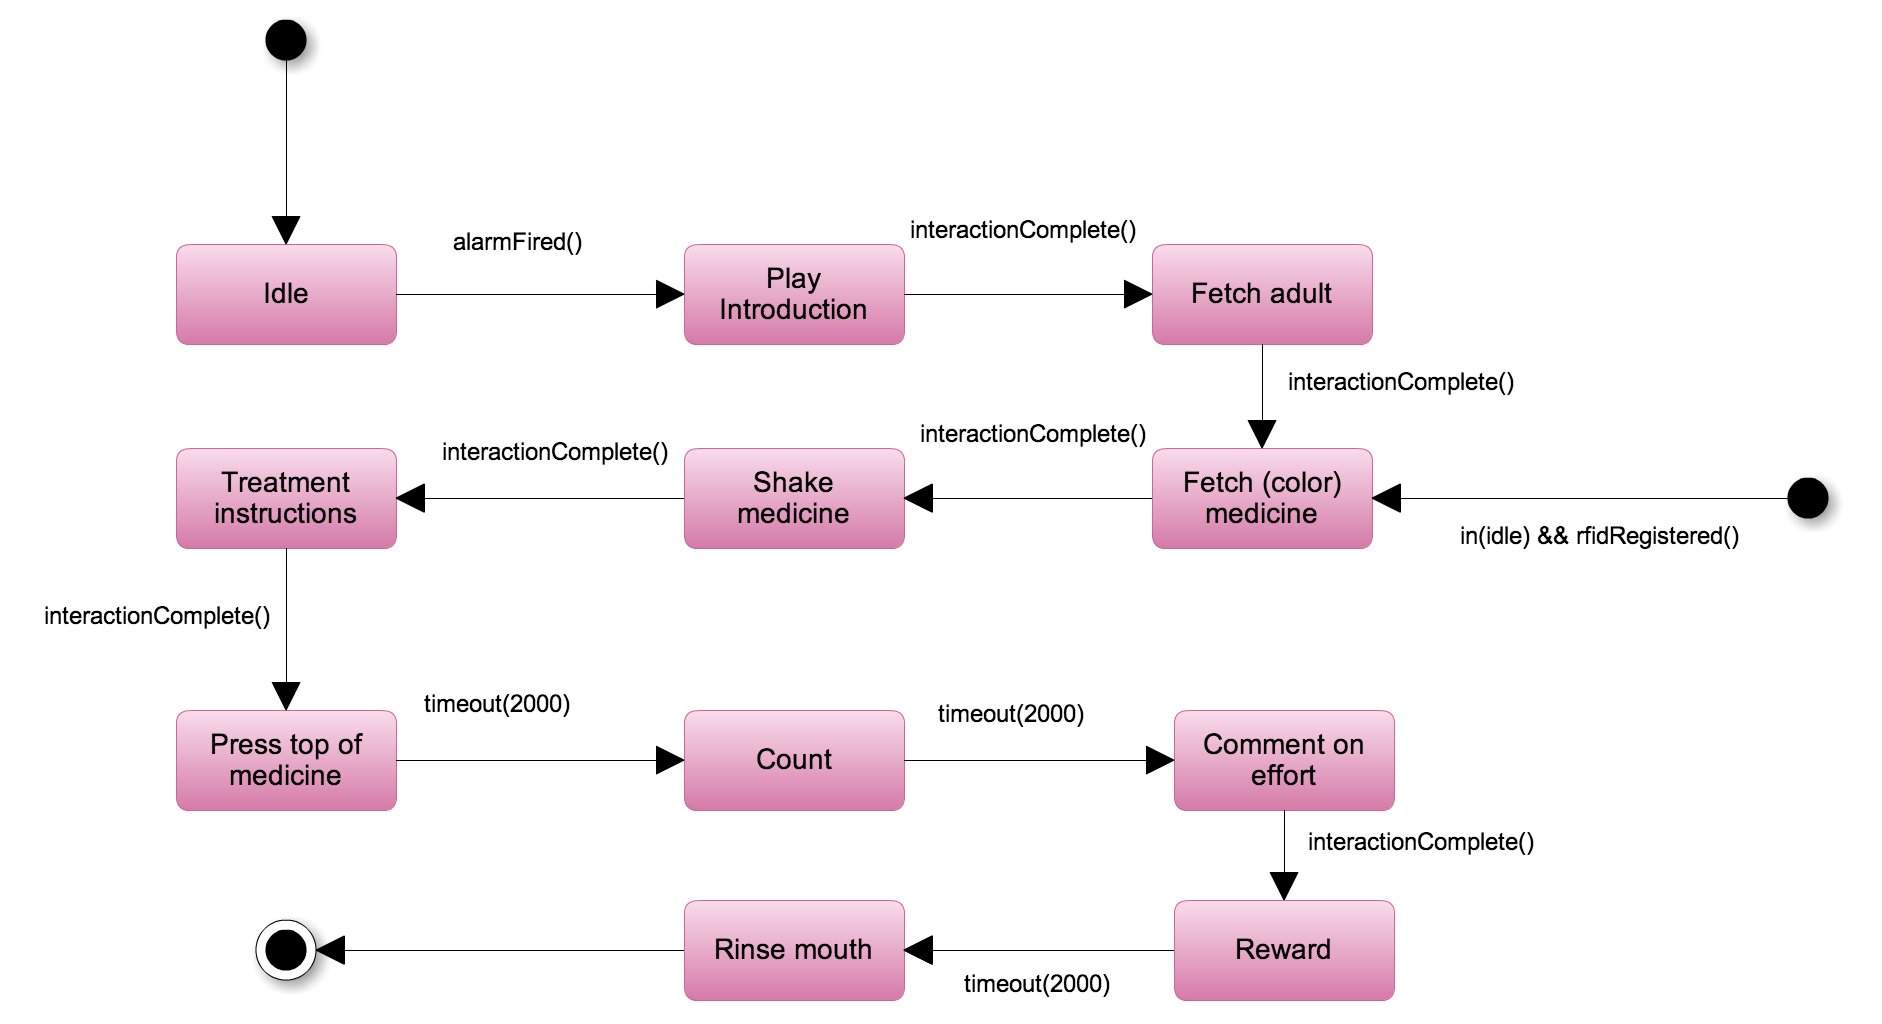
\includegraphics[width=0.6\paperwidth]{Pictures/statediagram.png}
	\caption{AsthmaBuddy State Diagram.}
	\label{fig:asthmabuddy_statediagram}
\end{figure}
 
\section{Prototype number 1}
Our first prototype was a ``dumb'' version with the purpose of testing out different methods of interaction. We wanted to get as many different experiences as possible, in order to find what kids are thinking as ideal. Even though some of the interaction methods are infeasible to implement during the thesis, we wanted to know what children think of as fun interaction. We also found it important that children were motivated to give us honest results, so we wanted to give them freedom to be innovative and let their imagination play a part.  

As a result, the first prototype was a simple state machine. The usability test was performed on NSEP's usability lab. Terje R\o sand sat in the backroom filming the sequence, while having a computer with ssh-connection to AsthmaBuddy. Whenever he observed that the children performed the method of interaction, he pressed enter in order for AsthmaBuddy to progress it's medication sequence. 
 
For the first prototype we tried out the following types of interaction with AsthmaBuddy:
\begin{enumerate}
	\item{Give AsthmaBuddy a ``High Five''}
	\item{Hold AsthmaBuddy's hand}
	\item{Hold smartphone close to AsthmaBuddy's belly}
	\item{Press AsthmaBuddy's nose}
	\item{Press AsthmaBuddy's belly}
	\item{Hold medicine close to AsthmaBuddy's mouth}
	\item{Hold RFID-chip close to \buddy{}'s nose}
	\item{Hold RFID-chip close to \buddy{}'s belly}
	\item{Clap your hands}
\end{enumerate}


\section{Prototype number 2}


\section{Further improvements}

 
%\subsection{Dealing with Bellotti's Challenges}
%\label{sec:handling-challenges}
%The main challenges Bellotti has identified (see Table \ref{tab:tuichallenges}) is \emph{``How to control or cancel system action in progress''} and \emph{``How to specify and select a possible object for action''}. We have previously stated that there are two cases in which a child will take their medicine, \emph{by need} and \emph{as a preventive measure}. An issue that could rise is how to detect when a child needs to take a medicine by need. Preventive medicines will fire alarms on AsthmaBuddy, and the child automatically knows that the system is ``awake''. However, when a child needs to take it by need, there is no other intuitive way to show that the AsthmaBuddy is awake than using LED-lights, which are the key for the system to work. Thus, the solution to the second challenge is usage of LED-lights. Cancelling operations, however, is difficult to find a ``good'' solution from a usability standpoint. 

%For instance, if AsthmaBuddy starts counting seconds on a treatment before a child is ready, there will be a need to reset this counter, or basically at any point during a treatment, go back to the last step. At the moment, the only solution we are able to see at this problem is to use RFID-chips to backtrack, modelling the treatment process as a statemachine. 
 